\section{Single-layer antireflection coating}

Beyond the idealised index-matched case of the previous section, the
quarter-wave AR formula predicts a finite residual reflectance whenever
the film index is not exactly $\sqrt{n_0 n_s}$. The benchmark here is a
magnesium-fluoride film ($n_f = 1.38$) on crown glass ($n_s = 1.52$) in
air ($n_0 = 1.00$) at the design wavelength
$\lambda_0 = \SI{550}{\nano\metre}$. The analytical optimum thickness and
residual reflectance are
\begin{align}
  d_{\rm opt} &= \frac{\lambda_0}{4 n_f} \approx \SI{99.6}{\nano\metre}, \label{eq:ar-d}\\[2pt]
  R_{\min}    &= \left(\frac{n_0 n_s - n_f^{2}}{n_0 n_s + n_f^{2}}\right)^{2}. \label{eq:ar-Rmin}
\end{align}
$R_{\min}$ is the exact reflectance of the stack at $\lambda_0$ when
$d = d_{\rm opt}$; it vanishes only in the index-matched limit
$n_f^{2} = n_0 n_s$.

Two independent scans are performed: panel (a) fixes the wavelength at
$\lambda_0$ and sweeps the film thickness from $0$ to \SI{300}{\nano\metre}
on a 601-point grid, locating the analytic minimum; panel (b) fixes the
thickness at $d_{\rm opt}$ and sweeps the wavelength across
\SIrange{400}{700}{\nano\metre}, overlaying the bare-substrate reflectance
for reference.

\begin{center}
\begin{tikzpicture}
  \fill[black!4] (0, 0) rectangle (5, 1.6);
  \fill[green!10] (0,-0.7) rectangle (5, 0);
  \fill[blue!6]  (0,-1.9) rectangle (5,-0.7);
  \draw[thick] (0,0) -- (5,0);
  \draw[thick] (0,-0.7) -- (5,-0.7);
  \node[lbl, anchor=east] at (4.9, 1.2) {air};
  \node[lbl, anchor=east] at (4.9,-0.35) {MgF$_2$, $d_{\rm opt}$};
  \node[lbl, anchor=east] at (4.9,-1.4) {glass};
  \raysketch{1.6}{0}{f}
\end{tikzpicture}
\end{center}

\begin{figure}[!htbp]
  \centering
  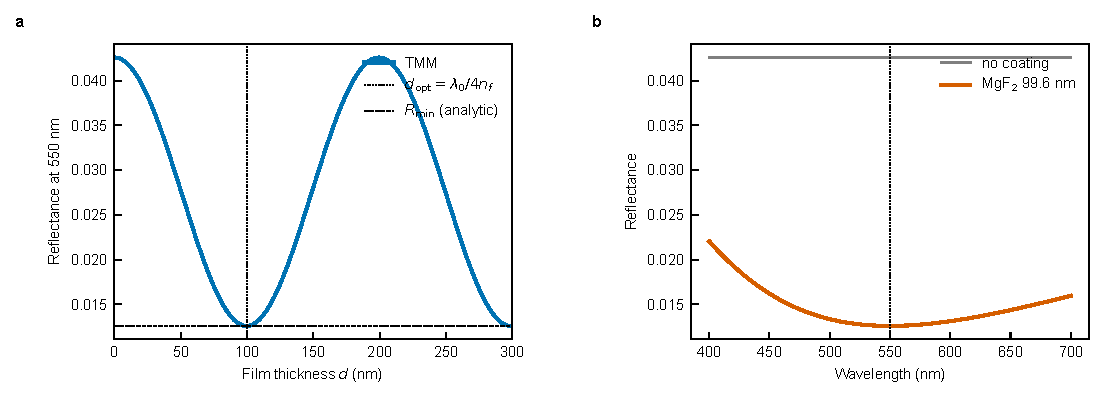
\includegraphics[width=\textwidth]{06_antireflection_coating.pdf}
  \caption{(a) Reflectance as a function of film thickness at $\lambda_0 = \SI{550}{\nano\metre}$, touching the analytic $R_{\min}$ at $d = d_{\rm opt}$. (b) Reflectance against wavelength at the optimum thickness, with the bare-substrate curve overlaid for comparison.}
  \label{fig:ar}
\end{figure}

The minimum of the TMM thickness scan falls exactly
on~\eqref{eq:ar-Rmin} with
$|R_{\rm TMM}(d_{\rm opt}, \lambda_0) - R_{\min}| \approx \num{7e-18}$, and
the wavelength scan shows the familiar broadband V-shape touching the
analytic $R_{\min}$ only at the design wavelength. The residual
reflectance (here $R_{\min} \approx \num{1.3e-2}$) is a pure consequence of
the index mismatch between MgF$_2$ and the glass--air geometry; broadening
the AR spectrally requires multilayer designs, which are addressed by the
Bragg and bandpass examples below.


